\documentclass[aspectratio=1610]{ctexbeamer}
\usetheme{Berlin}
\usepackage{xeCJK}
\usepackage{multirow}
\usepackage{graphicx}
\usepackage{booktabs} % for better table formatting
\usepackage{geometry} % for adjusting page layout
% \usepackage{enumitem} % for customizing lists
\usepackage{hyperref} % for clickable links and references
\usepackage{subcaption}
\usepackage{tikz}
\usepackage{amsmath}
\usetikzlibrary{quantikz}
\setbeamertemplate{itemize item}[ball] % Can be circle, square, etc.
\setbeamertemplate{itemize subitem}[default] % Can be ball, triangle, etc.
\title[学位论文答辩]{基于TDD的量子模型检测中的可达性分析}
\subtitle{硕士学位论文答辩}
\author[Gc]{高丁超\\ 导师:应圣钢}
\institute[ISCAS]{中国科学院软件研究所}
\AtBeginSection[]{
  \ifthenelse{\equal{\secname}{End}}{}{ % Checks if the section name is "End"
    \begin{frame}<beamer> % Only creates the frame if the section is not "End"
        \frametitle{目录}
        \tableofcontents[currentsection]
    \end{frame}
  }
}

\begin{document}
\begin{frame}[plain]
    \titlepage
    \begin{figure}
        \centering
        \begin{subfigure}[c]{0.4\textwidth}
            \centering
            \includegraphics[height= 2cm]{Img/iscas.png}
        \end{subfigure}
        \qquad
        \begin{subfigure}[c]{0.4\textwidth}
            \centering
            \includegraphics[height= 2cm]{Img/ucas.jpg}
        \end{subfigure}
    \end{figure}
    %  Title page
\end{frame}
\begin{frame}
    \frametitle{目录}
    \tableofcontents
\end{frame}

\section{背景介绍}

\begin{frame}
    \begin{itemize}
        \item \textbf{标题:} 基于张量网络的量子模型检测中的可达性分析
        \item \textbf{总结:}
        \begin{itemize}
            \setlength\itemsep{1em} % Set item separation here, for subitems
            \item \textit{问题:} 如何在量子系统中验证命题。
            \item \textit{解决方案:} 采用量子模型检测。
            \item \textit{挑战:} 原有的方法随着量子比特数量的增加,资源需求指数级增长。
            \item \textit{方法:} 引入新的数据结构TDD对量子算法进行表示,同时实现了优化算法进一步减少了时间消耗。
        \end{itemize}
    \end{itemize}
\end{frame}

\begin{frame}{量子计算的关键概念}
    \begin{itemize}
        % //TODO: add figure 
        \item \textbf{量子比特(Qubits):} the quantum version of the classic binary
        \item \textbf{叠加态(Superposition):} $|\psi\rangle = \alpha |0\rangle + \beta |1\rangle=\left[\begin{array}{r}\alpha \\\beta\end{array}\right]$
        \item \textbf{纠缠(Entanglement):}$|\Psi\rangle = \frac{1}{\sqrt{2}}(|00\rangle+|11\rangle)$
        \item \textbf{量子门(Quantum Gates)} 
    \end{itemize}
\end{frame}
\begin{frame}{量子门操作例子}
    \begin{itemize}
        \item \textbf{单量子门例子:}$X=\left[\begin{array}{rr}0 & 1 \\1 & 0 \end{array}\right],Y=\left[\begin{array}{rr}0 & -i \\i & 0 \end{array}\right],Z=\left[\begin{array}{rr}1 & 0 \\0 & -1 \end{array}\right],H=\frac{1}{\sqrt{2}}\left[\begin{array}{rr}1 & 1 \\1 & -1 \end{array}\right]$ 
        \item \textbf{多量子门例子:} $\text { CNOT }=\left[\begin{array}{llll}
            1 & 0 & 0 & 0 \\
            0 & 1 & 0 & 0 \\
            0 & 0 & 0 & 1 \\
            0 & 0 & 1 & 0
            \end{array}\right]$
        \item \textbf{测量,比如$Z$基测量:}状态为$|0\rangle$输出$1$,状态为$|1\rangle$输出$-1$。
    \end{itemize}
\end{frame}
\begin{frame}{量子计算例子}
    \begin{figure}[h]
      \centering
      \scalebox{1.1}{
      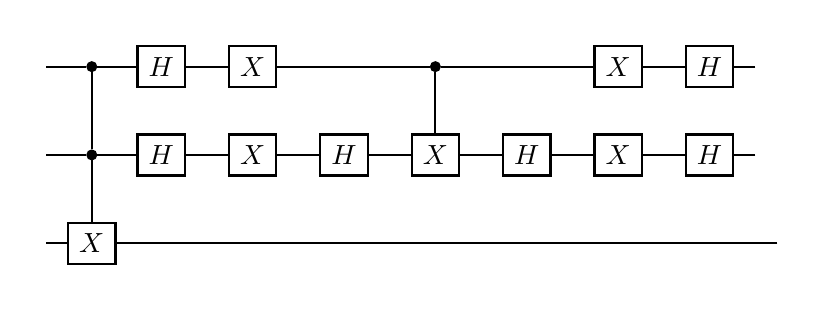
\begin{tikzpicture}
      \node at (0,0) [anchor=north]{
      \begin{quantikz}[column sep=0.28cm,row sep=0.6cm]
      &\ctrl{1}&\gate{H}&\qw&\gate{X}&\qw&\qw&\qw     &\ctrl{1}&\qw&\qw&\qw     &\gate{X}&\qw&\gate{H}&\qw \\
      &\ctrl{1}&\gate{H}&\qw&\gate{X}&\qw&\gate{H}&\qw&\gate{X}&\qw&\gate{H}&\qw&\gate{X}&\qw&\gate{H}&\qw \\
      &\gate{X}&\qw     &\qw     &\qw     &\qw     &\qw     &\qw     &\qw     &\qw&\qw&\qw&\qw&\qw&\qw&\qw&\qw 
      \end{quantikz}};
      \end{tikzpicture}
      }
      \label{fig:cir}
      \caption{Grover\_3算法的电路。}
    \end{figure}
\end{frame}
\begin{frame}{研究背景}
    \begin{itemize}
        \item<1-> 量子计算的快速发展
        \begin{itemize}
            \item 规模化拓展
            \begin{itemize}
                \item IBM: Condor \textbf{1121}; 中科大: 九章三号 \textbf{255}
            \end{itemize}
            \item 容错计算
            \begin{itemize}
                \item IonQ: \textbf{29}; QuEra:  \textbf{48}
            \end{itemize}
        \end{itemize}
        \item<2-> 现有验证方法
        \begin{itemize}
            \item 模型检测自动化程度高,但存在资源爆炸的问题
            \item 定理证明处理复杂问题有明显优势,但自动化程度低
        \end{itemize}
    \end{itemize}
\end{frame}
\begin{frame}{量子迁移系统}
    \begin{columns}[T] % The "T" option aligns the columns content at the top

        % Column for itemized list
        \begin{column}{.6\textwidth}
            \begin{itemize}
                \item  \textbf{迁移系统(transition system):} $(S, I, \Sigma, T)$
                \begin{equation}
                  where
                  \begin{cases}
                    x = x_1, \cdots, x_n\\
                    y = y_1, \cdots, y_n\\
                    \sigma = \sigma_1, \cdots, \sigma_m
                  \end{cases}
                  \notag
                \end{equation}
                \item \textbf{量子迁移系统:} $(\mathcal{H}, \mathcal{H}_0, Act, \{U_\alpha,\alpha\in Act\})$
            \end{itemize}
        \end{column}
    
        % Column for figure
        \begin{column}{.3\textwidth}
          \begin{figure}
            \centering
            \includegraphics[width=\textwidth]{Img/transition.png}
          \end{figure}
        \end{column}
    
      \end{columns}
    % //TODO: add figure
\end{frame}
\begin{frame}{可达性问题}
    \begin{figure}
        \includegraphics[width=.6\textwidth]{Img/eventually.png}
    \end{figure}
    \begin{figure}
        \includegraphics[width=.6\textwidth]{Img/eventuallyalways.png}
    \end{figure}
    \begin{figure}
        \includegraphics[width=.6\textwidth]{Img/alwayseventually.png}
    \end{figure}
  \end{frame}
%   \begin{frame}{量子逻辑}
%     \begin{itemize}[itemsep=18pt]
%         \item \textbf{子集关系 \( \subseteq \) 在 \(S(\mathcal{H})\) 中:} 偏序关系,表示蕴涵。
%         \item \textbf{正交补 \( \mathcal{X}^\perp \):} 表示否定。
%         \item \textbf{闭合于交集:} \( \bigcap_{i} \mathcal{X}_{i} \in S(\mathcal{H}) \),表示合取。
%         \item \textbf{子空间的并集:} \( \bigvee_i \mathcal{X}_i = \text{span} \left( \bigcup_i \mathcal{X}_i \right) \),解释为析取。
%     \end{itemize}
% \end{frame}

\begin{frame}{量子模型检测例子}
    \begin{figure}[h]
        \centering
        \scalebox{0.8}{
        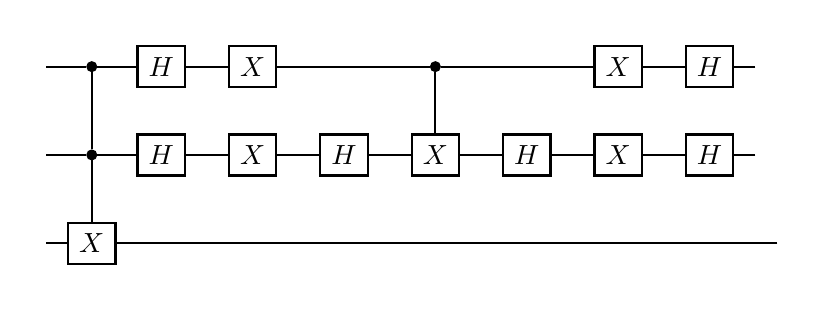
\begin{tikzpicture}
        \node at (0,0) [anchor=north]{
        \begin{quantikz}[column sep=0.28cm,row sep=0.6cm]
        &\ctrl{1}&\gate{H}&\qw&\gate{X}&\qw&\qw&\qw     &\ctrl{1}&\qw&\qw&\qw     &\gate{X}&\qw&\gate{H}&\qw \\
        &\ctrl{1}&\gate{H}&\qw&\gate{X}&\qw&\gate{H}&\qw&\gate{X}&\qw&\gate{H}&\qw&\gate{X}&\qw&\gate{H}&\qw \\
        &\gate{X}&\qw     &\qw     &\qw     &\qw     &\qw     &\qw     &\qw     &\qw&\qw&\qw&\qw&\qw&\qw&\qw&\qw 
        \end{quantikz}};
        \end{tikzpicture}
        }
        \label{fig:cir}
        \caption{Grover\_3算法的电路。}
    \end{figure}
    \begin{itemize}
        \item oracle为ccx,即$O|x\rangle|y\rangle = |x\rangle|f(x)\oplus y\rangle $,$f(x)=x_1\wedge x_2$。
        \item \textbf{model:} $(\mathcal{H}_8, S = span\{|++-\rangle,|11-\rangle\}, \{1\}, {\mathcal{T}_1})$, $\mathcal{T}_1 =(2|\Psi\rangle\langle \Psi| - I)O$ 
        \item \textbf{property:} $\mathcal{T}_1(S)=S$
    \end{itemize}
\end{frame}

% \begin{frame}{量子模型检测例子}
%     \begin{figure}
%       \includegraphics[height=3.5cm]{Img/cir_coum.pdf}
%       \caption{一个量子通信协议例子,其中$|\Psi\rangle = \frac{1}{\sqrt{2}}(|00\rangle+|11\rangle)$}
%     \end{figure}
% \end{frame}
% \begin{frame}{量子模型检测例子}
%     \begin{figure}
%         \centering
%         \begin{subfigure}{0.3\textwidth}
%           \includegraphics[width=\textwidth]{Img/rus_s.pdf}
%         \end{subfigure}
%         \quad
%         \begin{subfigure}{0.3\textwidth}
%           \includegraphics[width=\textwidth]{Img/rus_T.pdf}
%         \end{subfigure}
%         \caption{两个rus电路}
%     \end{figure}
% \end{frame}
\begin{frame}{张量决策图(TDD)}
    \begin{itemize}
        \item \textbf{TDD 定义:} 由节点集 $V$、边集 $E$、索引函数 $index$、值函数 $value$、低高边映射 $low/high$ 和权重 $w$ 组成。
        \item
        \begin{itemize}
            \item 节点集$V$分为非终端节点 $V_N$ 和终端节点 $V_T$,且有唯一根节点 $r_{\mathcal{F}}$。
            \item 边集$E$包含所有低边 $\left(v,low(v)\right)$ 和高边 $\left(v,high(v)\right)$。
            \item 索引函数$index$ 分配索引,值函数$value$ 赋予终端节点复数值,$w$ 为边赋权重,特别是根边权重 $w_{\mathcal{F}}$。
        \end{itemize}
    \end{itemize}
\end{frame}

\begin{frame}{TDD例子}
    % //TODO: add 
    \begin{figure}
        \begin{subfigure}{0.4\textwidth}
            \includegraphics[height=3.5 cm]{Img/matrix_of_tdd.pdf}
            \label{fig:mat_P}
        \end{subfigure}
        \qquad
        \qquad
        \qquad
        \begin{subfigure}[c]{0.4\textwidth}
            \centering
            \includegraphics[height=6cm]{Img/tdd_ex.pdf}
            \label{fig:tdd_P}
        \end{subfigure}
        \label{fig:P}
        \caption{可以用10个TDD节点表示一个$8*8$的矩阵。其中TDD虚线表示低点,实线表示高边。}
    \end{figure}
\end{frame}
% \begin{frame}{相关工作效率比较}
%     \begin{figure}
%         \includegraphics[height=4cm]{Img/tdd-compare.pdf}
%         \caption{应用不同技术对QFT算法进行模拟的时间对比}
%     \end{figure}
%     \begin{center}
%         \begin{itemize}
        
%             \item TDD No part,TDD part I, TDD part II为不同的TDD收缩算法。 
%             \item QMDD为量子多值决策图,是一种常用的模型检测方法。
%             \item TN为Google的tensro network,是一种常用的张量方法。
%         \end{itemize}
%     \end{center}
% \end{frame}
% \begin{frame}{相关工作-QMDD}
%     \begin{columns}[T] % The "T" option aligns the columns content at the top

%         % Column for itemized list
%         \begin{column}{.6\textwidth}
%             \begin{figure}
%                 \includegraphics[height=4cm]{Img/QMDD_b.png}
%                 \caption{一个QMDD的示例。}
%             \end{figure}
%         \end{column}
%         \begin{column}{.4\textwidth}
%             \hspace{80pt}
%             \begin{itemize}
%                 \item TDD只有高边和低边,表示更简洁。
%             \end{itemize}
%         \end{column}
        
%     \end{columns}
%   \end{frame}
\section{研究内容}
\begin{frame}{解决方案简介:}
    \begin{itemize}
        \item \textbf{研究问题:}
        \item \textbf{基本方法:}将转移关系和初态转化为TDD表示,然后计算系统的状态转移。
        \item \textbf{改进算法:}
        \begin{itemize}
            % \item //TODO: add DD based
            \item \textbf{addition partition:} 寻找依赖最多的索引项,从而分割线路。
            \item \textbf{contraction partition:}通过预设的参数进行线路分割。
        \end{itemize}
        \item \textbf{创新点:}
        \begin{itemize}
            \item 通过TDD,可以自动化的验证更大规模的量子算法。
            \item 通过C++重构,实现了比过去TDD更好的运行效率。
        \end{itemize}
    \end{itemize}
\end{frame}

\begin{frame}{adddition partition}
    \begin{itemize}
        \item 将量子电路转换为索引依赖图G。
        \item 通过图G的连通度选择索引进行电路分割。
    \end{itemize}
    \begin{figure}
        \centering
        \includegraphics[height=4cm]{Img/cir_index_graph.pdf}
        \caption{Grover\_3 电路的索引依赖图。对索引项$x_3^1,x_3^2$进行线路分割,效果更好。}
    \end{figure}
\end{frame}
\begin{frame}{Contraction partition}
    \begin{itemize}
        \item 确定预设参数 k1 和 k2。
        \item 分割电路,每部分包括最多 k1 个量子比特,连接最多 k2 个多比特门。
    \end{itemize}
    \begin{figure}
        \centering
        \includegraphics[height=4cm]{Img/cir_contraction.pdf}
        \caption{对bit flip电路进行划分,其中k1=3,k2=2。}
    \end{figure}
\end{frame}
\section{研究结果}

\begin{frame}{工作成果}
    \begin{table}[]
        \scalebox{0.9}{
        \rule{0pt}{30pt}
        \begin{tabular}{l|ccc}
        benchmark & basic & addition& contraction \\\hline
        Grover 20       & $\sim$5分  & $\sim$4分 & $\sim$4秒  \\
        Quantum Fourier Transform 20           & $\sim$20分 & $\sim$11分 & $<$1秒 \\
        Quantum Random walk 20           & $\sim$6分 & $\sim$4分 & $\sim$15秒\\
        Bernstein-Vazirani 100           & $\sim$7秒 & $\sim$7秒 & $\sim$0.4秒 \\
        GHZ 500         & $\sim$3秒 & $\sim$1.5秒 & $\sim$1.7秒\\
        \end{tabular}
        }
        \caption{对不同量子算法计算一步迁移的时间消耗}
    \end{table}
    \begin{itemize}
        \item 对于有特殊结构的算法,如GHZ算法,addition partiton有更好的执行效率。
        \item 对于一般的电路,contraction partition的执行效率更好。
    \end{itemize}
\end{frame}
\begin{frame}{工作成果}
    \begin{itemize}
        \item 通过C++重构TDD,改进了内存管理,从而加快了计算效率。
    \end{itemize}
    \begin{figure}
        \includegraphics[height=5cm]{Img/python_c.pdf}
        \caption{用python 和 c++ 不同版本的TDD运行Bernstein-Vazirani算法的时间效率比较}
    \end{figure}
\end{frame}
\begin{frame}{未来计划}
    \begin{itemize}
        \item 应用等价性,可以化简数据结构。
        \item 结合优化算法与C++的优势,进一步提高执行效率。
    \end{itemize}
    \begin{figure}
    \centering
    \begin{subfigure}{0.4\textwidth}
        \centering
        \includegraphics[height=5cm]{Img/limdd.pdf}
    \end{subfigure}
    % Add an equal sign in the middle
    \hspace{1em} % Adjust space as needed
    \Large$=$
    \hspace{1em} % Adjust space as needed
    \begin{subfigure}{0.4\textwidth}
        \centering
        \includegraphics[height=5cm]{Img/limdd_reduce.pdf}
    \end{subfigure}
    \caption{Local Invertible Map-DD}
\end{figure}

\end{frame}

\section{学位论文修改情况}
\begin{frame}{盲审结果与修改情况}
    \begin{itemize}
        \item \textbf{审稿人意见}:优秀,良好,良好
        \item \textbf{表达规范性}:专有名词,引用学者称呼规范化
        \item \textbf{工作完整性}:算法的正确性保证
    \end{itemize}
\end{frame}
\section*{}
\begin{frame}
    \centering
    \Huge 谢谢
\end{frame}
\end{document}